\documentclass[useAMS,usenatbib]{mn2e}
\usepackage{footnote,graphicx,color,multirow,amsmath,url,amssymb,tabularx,amssymb}

% \hypersetup{
%     colorlinks,
%     citecolor=blue,
%     filecolor=black,
%     linkcolor=black,
%     urlcolor=black
% }

\def\lesssim{\mathrel{\hbox{\rlap{\hbox{\lower3pt\hbox{$\sim$}}}\hbox{\raise2pt\hbox{$<$}}}}}


\begin{document}

\title[Quenching Histories of Fast and Slow Rotators]{SDSS-IV MaNGA: The Quenching Histories of Fast and Slow Rotators}
\author[Smethurst et al. 2017]{R. ~J. ~Smethurst,$^{1,2}$ C. ~J. ~Lintott,$^{2}$ et al.
\\ $^1$ School of Physics and Astronomy, The University of Nottingham, University Park, Nottingham, NG7 2RD, UK
\\ $^2$ Oxford Astrophysics, Department of Physics, University of Oxford, Denys Wilkinson Building, Keble Road, Oxford, OX1 3RH, UK
}

\maketitle

\begin{abstract}
\end{abstract}

\begin{keywords}
galaxies -- photometry, galaxies -- statistics, galaxies -- morphology
\end{keywords}

\section{Introduction}\label{sec:intro}

Recent work studying the early-type galaxy population has revealed that is actually composed of two separate populations. The majority of early-types are rotationally supported \citep{emsellem11} with $\sim7$ times the number of regular (or `fast') rotators, with kinematic discs, than non-regular (or `slow') rotators, with dispersion dominated kinematics \citep{cappellari07, emsellem07}.  This has led to the proposal of a revision of Hubble's morphological classification scheme in the form of a `comb' \citep{cappellari16}, whereby the evolution of a disc galaxy from  disc to bulge-dominated takes place along a tine of the comb, until these systems become bulge dominated regular rotators. These regular rotators then evolve along the handle of the comb to become non-regular rotators. 

Dry major mergers are considered the most likely process to produce non-regular rotators \citep{duc11, naab14} as they can rapidly destroy the disc dominated nature of a galaxy \citep{toomre72}. This percentage is therefore also an estimate for the fraction of the galaxy population which have undergone a dry major merger, approximated by previous works to be $\sim10-20\%$ since $z\sim1$; \citep[][]{khochfar09}.

Regular rotators, are thought to be formed by the slow build up of a galaxy's bulge over time, until it eventually overwhelms the disc. This growth is thought to occur via gas-rich major and minor mergers \citep{duc11} which can produce a bulge dominated, rotationally supported galaxy, which would be visually classified as an early-type. Although these mechanisms do not completely destroy the disc of a galaxy, they do cause an eventual morphological change to a visually bulge-dominated system.

The majority of the early-type population resides on the red sequence, with little to no star formation occurring. If these two populations of early-type galaxies are formed by two different mechanisms, we should therefore also expect to find a difference in their star formation histories. Both major mergers and minor mergers have been postulated as quenching mechanisms, with major mergers thought to cause a much faster quench of the remnant galaxy than a minor merger. 

In this work we use a Bayesian star formation inference package, \textsc{starpy}~ to determine the quenching histories of a population of early-type galaxies, classified as either regular or non-regular rotators using data from the Mapping Nearby Galaxies at Apache (MaNGA) survey. We use broadband optical, $u-r$ and near-ultraviolet $NUV-u$ colours from SDSS and GALEX to infer both the time and rate that quenching occurs in each galaxy, before visualising the distribution of these parameters across the regular and non-regular populations. We aim to determine whether regular and non-regular rotating early-type galaxies quench at different rates. 

This paper proceeds as follows. In Section~\ref{sec:datamethods} we describe our data sources and our Bayesian inference method for determining the quenching histories. We present our results in Section~\ref{sec:results}. We discuss the implications of our results in Section~\ref{sec:discussion}. The zero points of all magnitudes are in the AB system. Where necessary, we adopt the WMAP Seven-Year Cosmology \citep{jarosik11} with $(\Omega_m , ~\Omega_\Lambda , ~h) = (0.26, 0.73, 0.71)$.



\section{Data and Methods}\label{sec:datamethods}

\subsection{SDSS \& GALEX Photometry}\label{sec:photom}

We obtain optical photometry from the Sloan Digital Sky Survey Data Release 7 (SDSS; \citealt{york00, abazajian09}). We utilise the Petrosian magnitude, {\tt petroMag}, values for the $u$ ($3543 \rm{\AA}$) and $r$ ($6231 \rm{\AA}$) wavebands provided by the SDSS DR7 pipeline \citep{stoughton02}. Further to this, we also required NUV ($2267 \rm{\AA}$) photometry from the GALEX survey \citep{martin05}. Observed fluxes are corrected for galactic extinction \citep{Oh11} by applying the \citet*{Cardelli89} law. We also adopt $k$-corrections to $z = 0.0$ and obtain absolute magnitudes from the NYU-VAGC \citep{blanton05, padmanabhan08, blanton07}.

\subsection{MaNGA Survey \& Data Reduction Pipeline}\label{sec:manga}


MaNGA is a multi-object IFU survey conducted with the $2.5~\rm{m}$ Sloan Foundation Telescope \citep{gunn06} at Apache Point Observatory (APO). By 2020 MaNGA will have acquired IFU spectroscopy for $\sim10000$ galaxies, all with $M_* > 10^9~\rm{M}_{\odot}$ and an approximately flat mass selection (Wake et al., in preparation). The target selection does not include any cuts on morphology, colour or environment. 

In order to obtain spectra, MaNGA makes use of the Baryon Oscillation Spectroscopic Survey (BOSS) spectrograph \citep{smee13}. The BOSS spectrograph provides continuous coverage between $3600~\AA$ and $10300~\AA$ at a spectral resolution $R \sim 2000$ ($\sigma_{\rm{instrument}} \sim 77 \rm{km}~\rm{s}^{−1}$).

Complete spectral coverage to $1.5 R_e$ is obtained for the majority of targets, though a subset have coverage to $2.5 R_e$. See \cite{bundy15} for an overview of the MaNGA survey. For a further description of the instrumentation used by MaNGA see \cite{drory15}. For a detailed description of the observing strategy see \cite{law15} and for  description of the survey design see \cite{yan16}. %Analysis of the prototype MaNGA (P-MaNGA) observations are presented in \cite{li15, wilkinson15, belfiore15}.

The raw data was processed by the MaNGA data reduction pipeline (DRP), which is discussed in detail \cite{law16}. The MaNGA DRP extracts, wavelength calibrates and flux calibrates all fibre spectra obtained in every exposure. The individual fibre spectra are then used to form a regular gridded datacube of $0.5''$ ‘spaxels’ and spectral channels. The spectra are logarithmically sampled with bin widths of $\log{\lambda} = 10^{-4}$. 

These datacubes are then analysed using the MaNGA data analysis pipeline (DAP); the development of which is ongoing and will be described in detail in Westfall et al. (in preparation). The primary output from the DAP are the MAPS files which provide 2D "maps" (i.e., images) of DAP measured properties, which include flux, stellar-continuum fits, absorption- and emission-line properties and spectral index measurements. The DAP also provides a measurement of a galaxy's ellipticity, $\epsilon$, and effective radius, $R_e$, which is used along with the specific angular momentum to classify galaxies as either regular or non-regular rotators (see Section~\ref{sec:mangasample}).

\subsection{Data sample}\label{sec:mangasample}

There are currently $2,777$ galaxies observed by the MaNGA survey and consequently are part of SDSS DR7. We cross-matched these galaxies with a radius of $3''$ to the GALEX survey in order to obtain NUV photometry (see Section~\ref{sec:photom}), resulting in $1,413$ galaxies. We shall refer to this as the \textsc{manga-galex} sample. 

In this study we wish to study the quenching histories of these galaxies, therefore we sub-select those galaxies which are below the `star forming sequence' (SFS\footnote{Sometimes referred to as the `'main'' sequence or star formation.}). Here we utilise the values quoted in the MPA-JHU catalogue \citep{kauffmann03, brinchmann04} which quantify the SFR of a galaxy using the $\rm{H}\alpha$ emission line observed in the SDSS fibre spectra and correct this for aperture bias using SDSS photometry to provide a galaxy wide SFR. Whilst we do not use this value to infer the SFHs of these galaxies (see Section~\ref{sec:starpy}), we do utilise them to select a sample of galaxies with SFRs more than $1\sigma$ below the SFS of \cite{peng10}. 

In this investigation we also focus on the different formation (and therefore quenching) histories of early-type galaxies and so utilise the morphological classifications of Galaxy Zoo 2 \citep[GZ2; ][]{lintott11, GZ2}. We select those galaxies classified as `smooth' by GZ2 users (i.e. with a debiased `smooth' vote fraction of $p_s \geq 0.8$).  These selections on morphology and SFR applied to the \textsc{manga-galex} sample result in a sample of $167$ quenching or quenched early-type galaxies, which we will refer to as the \textsc{q-etg} sample. The positions of these galaxies below the SFS are shown in Figure~\ref{fig:masvsfr}. 

\begin{figure}
\centering
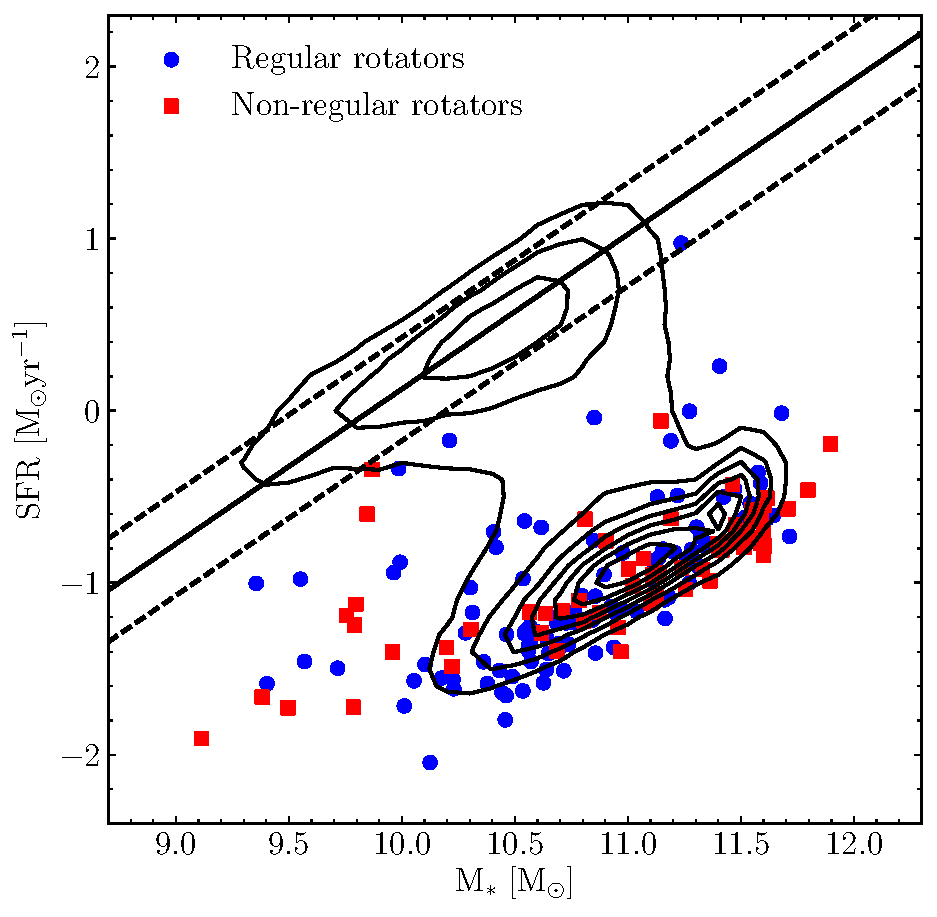
\includegraphics[width=0.475\textwidth]{../figures/nonSF_FR_SR_SFS_scatter.pdf}
\caption{Stellar mass against star formation rate for the~\textsc{q-etg}~sample split into regular (blue circles) and non-regular (red squares) rotators. Shown also are the contours for the entire MPA-JHU sample (black contours; i.e. SDSS DR7). The solid line shows the SFS as defined by \cite{peng10} at the average redshift of the \textsc{q-etg} sample with $\pm1\sigma$ shown by the dashed lines. Note that the galaxies in the \textsc{q-etg} sample are chosen to be more than $1\sigma$ below the SFS as defined at their observed redshift and stellar mass (see Section~\ref{sec:mangasample}).}
%KS Test between distributions?
\label{fig:masvsfr}
\end{figure}

In order to classify the galaxies in the \textsc{q-etg} sample as regular rotators or otherwise, we use the equation for specific stellar angular momentum as defined by \cite{emsellem07, emsellem11};
\begin{equation}
\lambda_R_e = \frac{\sum_{i=1}^{N} F_i\ R_i\ |V_i|}{\sum_{i=1}^{N} F_i\ R_i\ (V_i^2 + \sigma_i^2)^{1/2}}
\end{equation}	

where $F_i$ is the flux in the $i$th spaxel, $R_i$ the spaxel's distance from the galaxy centre (where $R_i < R_e$, the effective radius of a galaxy), $V_i$ the mean stellar velocity in that spaxel, $\sigma_i$ the stellar velocity dispersion in that spaxel and $N$ the total number of spaxels. In this work we use the python function provided in the MaNGA DAP to calculate $\lambda_R$ using the values of mean flux, radius, stellar velocity and stellar velocity dispersion (corrected for instrumental resolution effects) provided in the MAPS files generated by the MaNGA DAP (see Section~\ref{sec:manga}).

We classify galaxies in the \textsc{q-etg} sample as regular or non-regular rotators using the definition from \cite{cappellari16}:

\begin{equation}
\lambda_R_e < 0.08 + \epsilon_e/4 ~ \rm{with} ~ \epsilon_e < 0.4
\end{equation}

where $\epsilon_e$ is the ellipticity of a galaxy within it's effective radius, $R_e$. Using this definition reveals $106$ ($63\%$) regular rotators and $61$ ($37\%$) non-regular rotators. Velocity dispersion measurements in each spaxel of a galaxy were confirmed to be above the instrument resolution of $77~\rm{km}~\rm{s}^{-1}$. They are shown by their velocity maps in Figure~\ref{fig:evsl}. 

\begin{figure*}
\centering
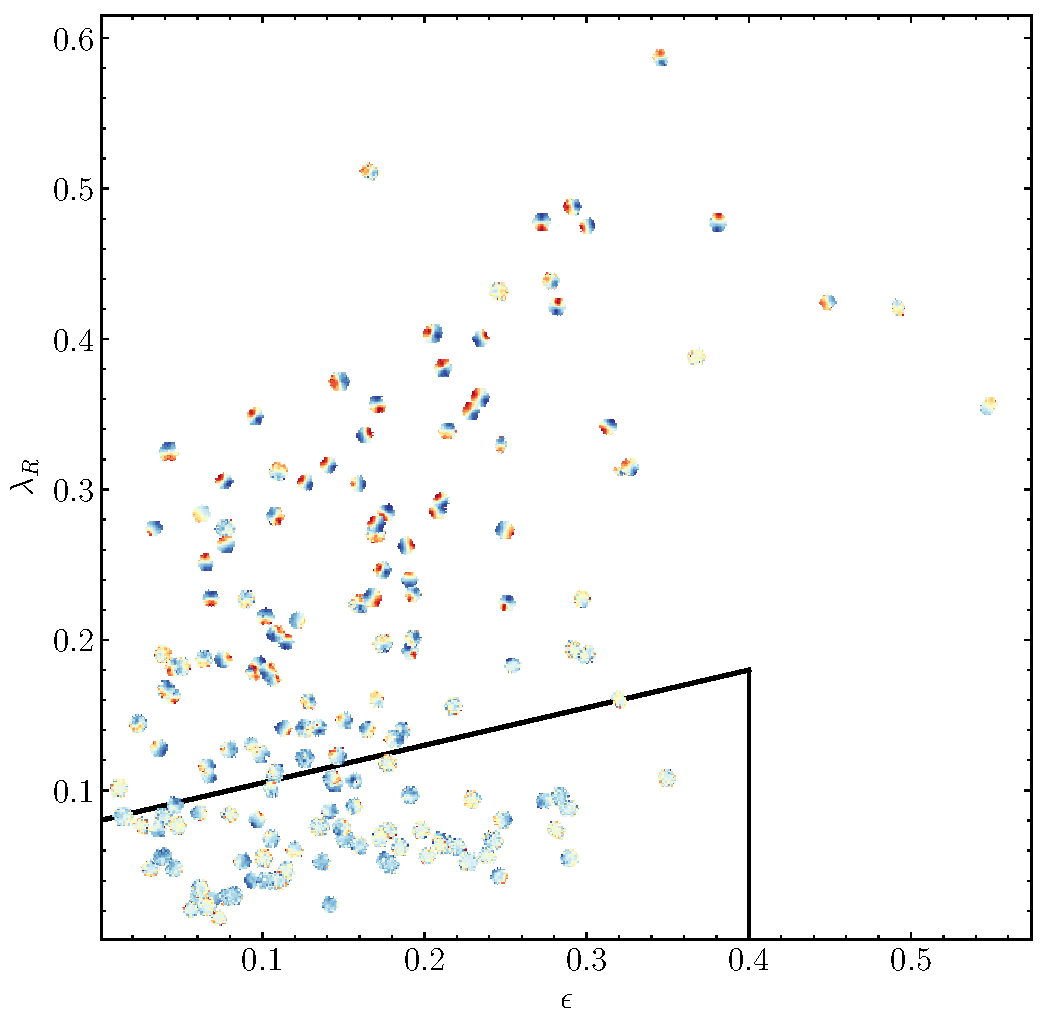
\includegraphics[width=\textwidth]{../figures/nonSF_ETGs_FR_SR_sample_orig_cmap_vel_maps.pdf}
\caption{Ellipticity versus stellar angular momentum for the quenching and quenched galaxies in the current observed MaNGA sample. Each point is shown by its stellar velocity map, each normalised to have the midpoint, between maximum and minimum measured velocity dispersions, shown by the colour yellow. We show the separation between regular (i.e. fast) and non-regular (i.e. slow) rotators from Cappellari (2016) with the black solid line.}
%KS Test between distributions?
\label{fig:evsl}
\end{figure*}

\subsection{STARPY}\label{sec:starpy}

\textsc{starpy}\footnote{Publicly available: \url{http://github.com/zooniverse/starpy}} is a \textsc{python} code which allows the derivation of the exponentially declining star formation history (SFH) of a single galaxy using  Bayesian Markov Chain Monte Carlo techniques \citep{emcee13}\footnote{\url{http://dan.iel.fm/emcee/}}. The code uses the solar metallicity stellar population models of \cite[][hereafter BC03]{BC03}, assumes a Chabrier IMF \citep{chabrier03} and requires the input of the observed $u-r$ and $NUV-u$ colours and redshift. No attempt is made to model for intrinsic dust. 

The SFH is described by an exponentially declining SFR described by two parameters; the time at the onset of quenching, $t_q~\rm{[Gyr]}$, and the exponential rate at which quenching occurs, $\tau~\rm{[Gyr]}$. Under the simplifying assumption that all galaxies formed at $t=0$ $\rm{ Gyr}$ with an initial burst of star formation, the SFH can be described as: 
\begin{equation}\label{sfh}
SFR =
\begin{cases}
i_{sfr}(t_q) & \text{if } t < t_q \\
i_{sfr}(t_q) \times exp{\left( \frac{-(t-t_{q})}{\tau}\right)} & \text{if } t > t_q 
\end{cases}
\end{equation}
where $i_{sfr}$ is an initial constant star formation rate dependent on $t_q$ \citep{schawinski14, smethurst15}.  A smaller $\tau$ value corresponds to a rapid quench, whereas a larger $\tau$ value corresponds to a slower quench. Note that a galaxy undergoing a slow quench is not necessarily quiescent by the time of observation. Similarly, despite a rapid quenching rate, star formation in a galaxy may still be ongoing at very low rates, rather than being fully quenched. This SFH model has previously been shown to appropriately characterise quenching galaxies \citep{Weiner06, Martin07, Noeske07,schawinski14}. 

We assume a flat prior on all the model parameters and model the difference between the observed and predicted $u-r$ and $NUV-u$ colours as independent realisations of a double Gaussian likelihood function (Equation 2 in \citealt{smethurst15}). We also make the simplifying assumption that the age of each galaxy, $t_\mathrm{age}$ corresponds to the age of the Universe at its observed redshift, $t_\mathrm{obs}$.

The probabilistic fitting methods to these star formation histories for an observed galaxy are described in full detail in Section 3.2 of \cite{smethurst15}, wherein the \textsc{starpy} code was used to characterise the morphologically dependence of the SFHs of $\sim126,000$ galaxies. Similarly, in \cite{smethurst16}, \textsc{starpy} was used to show the prevalence of rapid, recent quenching within a population of AGN host galaxies. 


An example posterior probability distribution output by \textsc{starpy} is shown for a single galaxy in Figure 5 of \cite{smethurst15}, wherein the degeneracies of the SFH model between recent, rapid quenching and earlier, slower quenching can clearly be seen. 

To study the SFH across a sample of many galaxies, these individual posterior probability distributions are stacked in $[t_q, \tau]$ space to give a single distribution for the sample. This is no longer inference but merely a method to visualise the results for a population of galaxies (see appendix section C in \citealt{smethurst16} for a discussion on alternative methods which may be used to determine the parent population SFH). These distributions will be referred to as the population SFH densities.

\section{Results}\label{sec:results}

We determine the population SFH densities for both the regular and non-regular rotators of the \textsc{manga-galex} sample. This is shown in Figure~\ref{fig:popfrvsr} for both the time that quenching occurs (left panel) and exponential rate of quenching (right panel) in the regular (black solid line) and non-regular (red dashed line) rotator populations. 

Whilst we cannot reject the hypothesis that the regular and non-regular rotators have the same distribution of quenching times, the distributions for the rate that quenching occurs for regular and non-regular rotators are significantly different. A KS-test on the two distributions gave a $p$-value of $p=0.0009$, which is a $3\sigma$ result.

\begin{figure*}
\centering
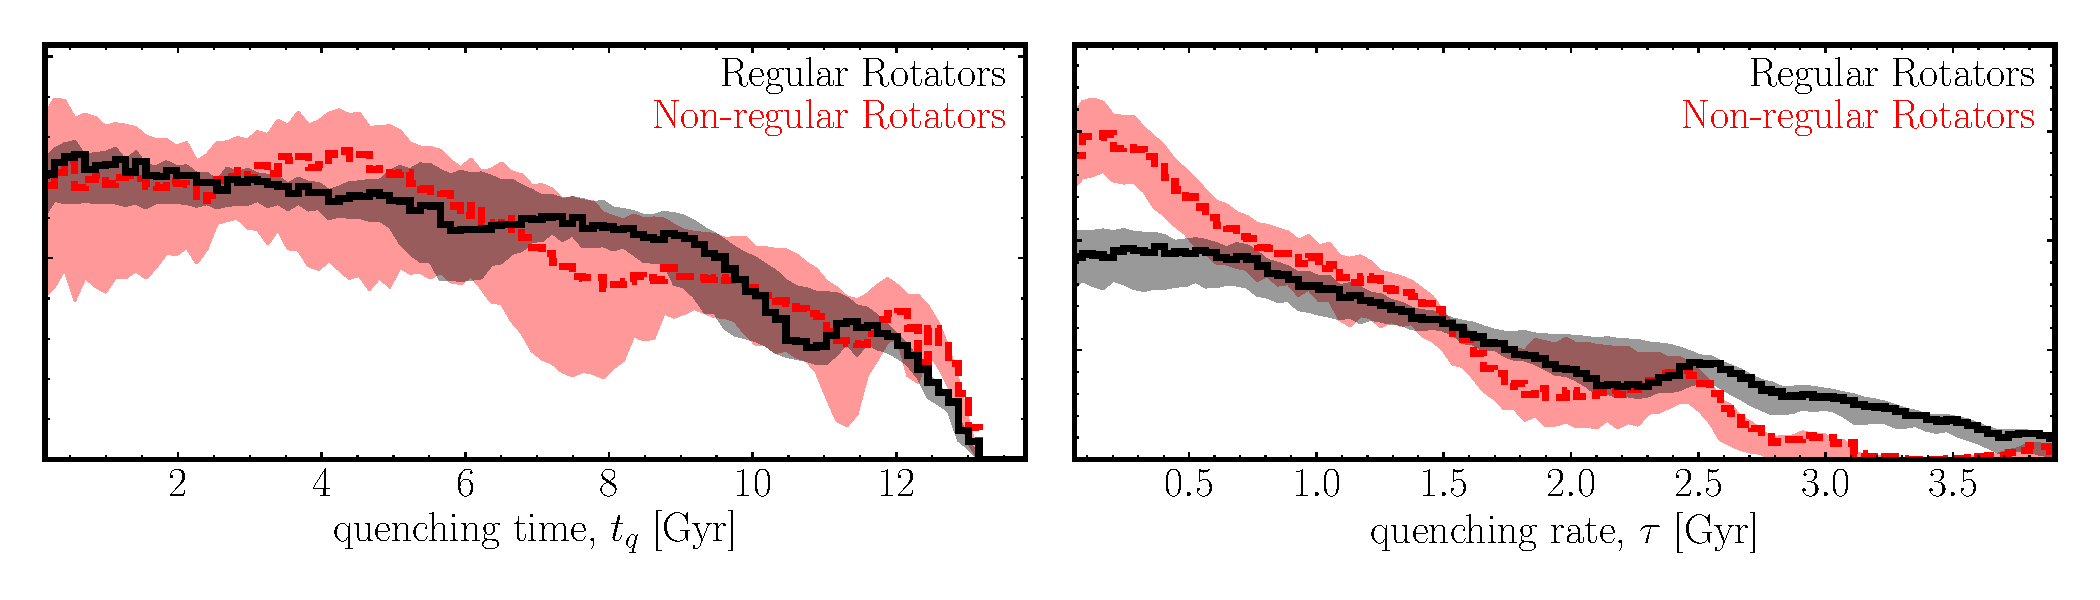
\includegraphics[width=\textwidth]{../figures/quenching_time_rate_FR_SR_NSF_C16.pdf}
\caption{Population densities for the time, $t_q$ (left) and exponential rate, $\tau$ (right) that quenching occurs in the \textsc{manga-nsf} sample for fast (black, solid) and slow (red, dashed) rotators. Shaded regions show the uncertainties on the distributions from bootstrapping. A KS-test between the $t_q$ distributions revealed that we cannot reject ($p=0.09$) the null hypothesis that the fast and slow rotators quench at the same time. However, a KS-test between the $\tau$ distributions revealed that we can reject ($p=0.0009$) the hypothesis that the fast and slow rotators quench at the same rate. This is a $3\sigma$ result, suggesting that slow rotators quench more rapidly.}
%KS Test between distributions?
\label{fig:popfrvsr}
\end{figure*}

\section{Discussion}\label{sec:discussion}

Regular and non-regular rotators are indeed separate populations quenched, and therefore formed, by different mechanisms. However, regular rotators can still quench at rapid rates along with slower rates. This ties in with the simulation results showing that discs can reform after major mergers. 

\bibliographystyle{mn2e}
\bibliography{refs}  

\end{document}
